\documentclass[12pt]{article}

\usepackage{amsmath}
\usepackage{amsthm}
\usepackage{amssymb}
\usepackage{mathrsfs}
\usepackage{setspace}
\usepackage{graphicx}
\usepackage{caption}
\usepackage{subcaption}
\usepackage{minted}

\newcommand{\w}{\omega}
\renewcommand{\a}{\alpha}
\renewcommand{\d}{\delta}
\newcommand{\s}{\sigma}
\newcommand{\e}{\epsilon}
\newcommand{\m}{\mu}

\newcommand{\inn}[1]{\left\langle #1 \right\rangle}
\newcommand{\norm}[1]{\left\Vert #1 \right\Vert}
\newcommand{\abs}[1]{\left\vert #1 \right\vert}

\newcommand{\real}{\mathbb{R}}
\newcommand{\nat}{\mathbb{Z}^+}

\begin{document}

\title{Homework 4}
\date{\today}
\author{Hunter Schwartz}
\maketitle

%\doublespacing

\textbf{Problem 1}

The trapezoid and Euler methods are implemented to numerically find the solution to the system as follows.

\begin{minted}[frame=lines,fontsize=\footnotesize,linenos]{python}
import numpy as np

# Problem statement
def f(t,Y):
    x,y,z = Y
    return np.array([-y, x, -100*(z - x**2 - y**2)])
    
def Df(t,Y):
    x,y,z = Y
    return np.matrix([[0, -1, 0],
                      [1, 0, 0],
                      [200*x, 200*y, -100]])

# Function to find root of for trapezoid method
def g(Y, Yj, tj, h):
    return Y - Yj - h/2*f(tj,Yj) - h/2*f(tj+h,Y)

def Dg(Y, Yj, tj, h):
    return np.eye(3) - h/2*Df(tj+h,Y)
        
# Problem parameters
Y0 = np.array([3, 0, 18])
h = 0.05
t = np.arange(0.2, 5, step=h)

# Trapezoid method
Y = np.empty([len(t), 3])
Y[0,:] = Y0

for j, tj in enumerate(t[0:-1]):
    Yj = Y[j,:]

    # Newton solve
    Yjp1 = Yj
    niters = 3
    for i in range(niters):
        gi = g(Yjp1, Yj, tj, h)
        Dgi = Dg(Yjp1, Yj, tj, h)
        s = np.linalg.solve(Dgi, gi)
        Yjp1 = Yjp1 - s
        
    Y[j+1,:] = Yjp1
    
# Euler's method
Z = np.empty([len(t),3])
Z[0,:] = Y0

for j, tj in enumerate(t[0:-1]):
    Z[j+1,:] = Z[j] + h*f(tj,Z[j])
\end{minted}

Plots of the resulting solutions are included below.

\begin{figure}[h]
\centering
\begin{subfigure}{.5\linewidth}
  \centering
  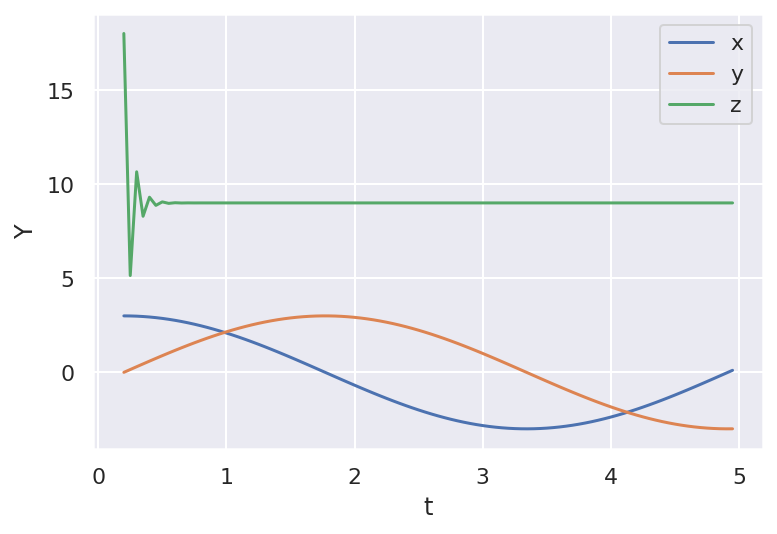
\includegraphics[width=\linewidth]{trapezoid.png}
\end{subfigure}%
\begin{subfigure}{.5\linewidth}
  \centering
  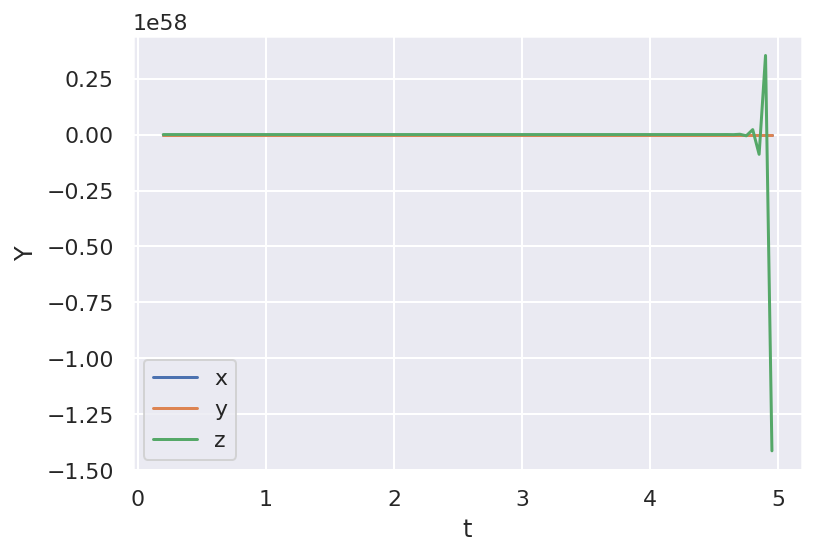
\includegraphics[width=\linewidth]{euler.png}
\end{subfigure}
\caption{Comparison of the solution found by the trapezoid method (left) and the solution of Euler's method (right).}
\end{figure}

\begin{figure}[h]
\centering
\begin{subfigure}{.5\linewidth}
  \centering
  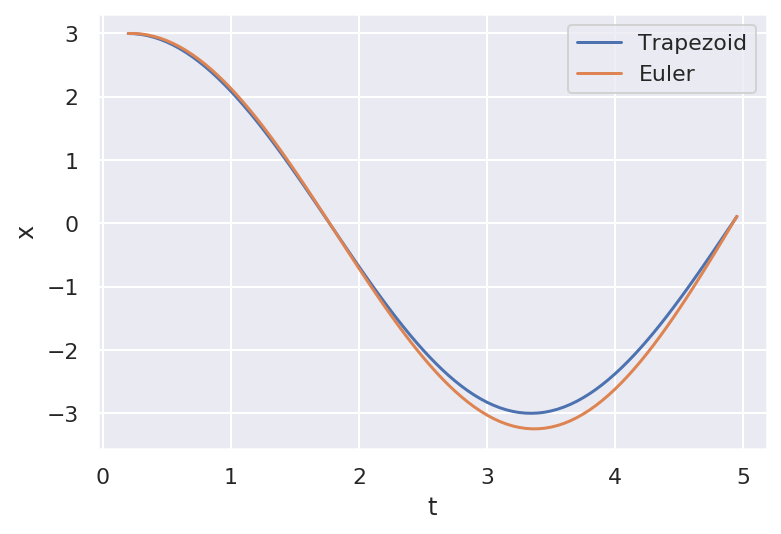
\includegraphics[width=\linewidth]{x.png}
\end{subfigure}%
\begin{subfigure}{.5\linewidth}
  \centering
  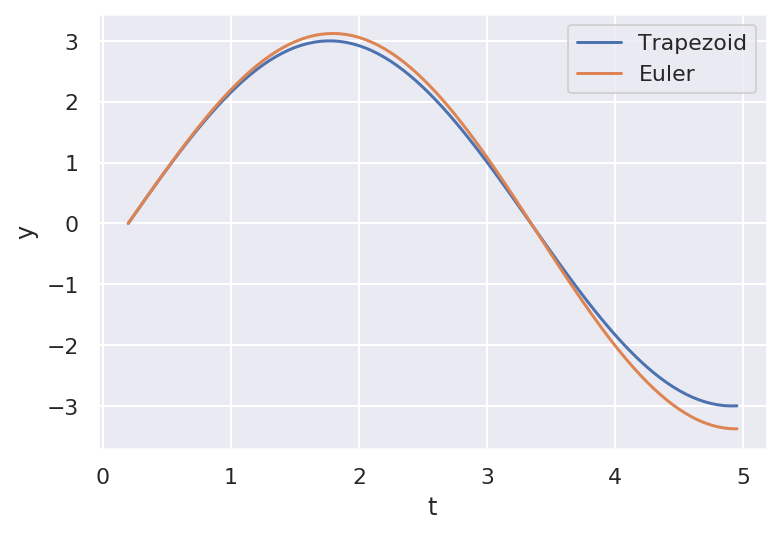
\includegraphics[width=\linewidth]{y.png}
\end{subfigure}
\begin{subfigure}{\linewidth}
  \centering
  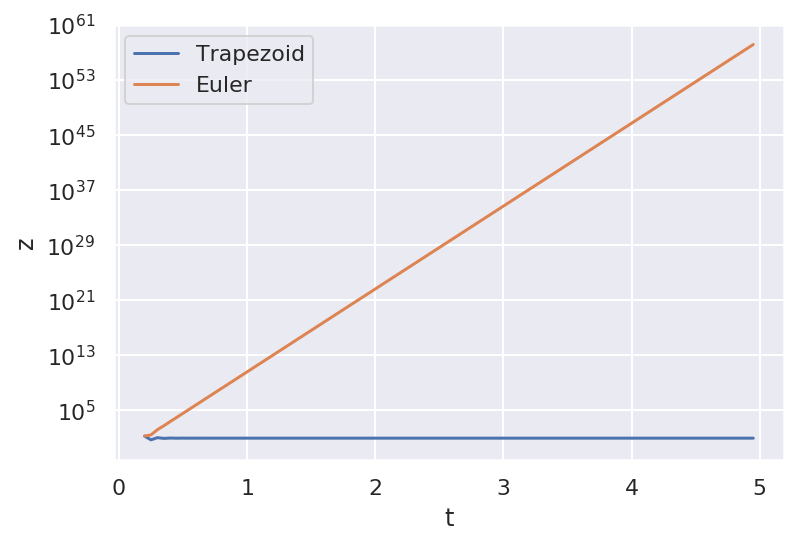
\includegraphics[width=.5\linewidth]{z.png}
\end{subfigure}
\caption{Dimension-wise comparison between the trapezoid and Euler's methods. The $z$ axis is scaled logarithmically.}
\end{figure}

The equations for $x$ and $y$ are decoupled from $z$, so they evolve independently in a now familiar way, such that $x^2 + y^2$ is constant. When $z = x^2 + y^2$, we have $z' = 0$, so $z$ will be stable if ever $z = x^2 + y^2$. Figure 1 demonstrates this in the solution of the trapezoid method, with $x,y$ sinusoidal and $z$ finding its way somewhat erratically to a resting state. In contrast, the solution to Euler's method grows larger with $t$ until $z$ is on the order of $10^{58}$. This is a reflection of the fact that Euler's method is stable for a much smaller selection of step sizes for a given problem, and the steps we are taking in this problem are too large for this stiff system.

In Figure 2, we can see that the solutions to $x$ and $y$ are very similar for both methods. We have seen before that Euler's method behaves well for this particular $x,y$ system, and since they are independent of $z$, we should see that Euler's method still solves for $x$ and $y$ well here. However, it is for the solution of $z$ that Euler's method fails dramatically, with the solution growing exponentially in $t$ whereas the actual solution is just a constant.

\end{document}